\section{Sharp analysis of low-rank kernel matrix approximations}
\begin{frame}
    \frametitle{Sharp analysis of low-rank kernel matrix approximations}

    \begin{itemize}
        \item \cite{bach2013sharp}
        \item Title: Sharp analysis of low-rank kernel matrix approximations.
        \item Author: Francis Bach.
        \item Year: 2013.
        \item Number of cites 316. 
    \end{itemize}
    
    Contribution interesting: 
    \begin{itemize}
        \item A kind of survey:
        \begin{itemize}
            \item kernel optimization, 
            \item analysis of column sampling approximation,
            \item randomized dimension reduction,
            \item theoretical analysis of predictive performance of kernel methods. 
        \end{itemize} 
        \item Number of columns in Nyström.   
    \end{itemize}
\end{frame}

\begin{frame}
    \frametitle{Contributions}

    \begin{itemize}
        \item The rank $p$ can be chosen to be linear in the degrees of freedom associated with the problem, a quantity which
        is classically used in the statistical analysis of such methods. 
        \item They present in Section 4.4 simple algorithms that have sub-quadratic running time complexity,
        and, for the square loss, provably exhibit the same predictive performance as classical algorithms than run in quadratic time (or more).
        
    \item They provide in Section 4.3 explicit examples of optimal values of the regularization parameters
and the resulting degrees of freedom, as functions of the decay of the eigenvalues of the kernel matrix, shedding some light in the joint computational/statistical trade-offs for choosing a
good kernel.
\item  They show that with kernels with fast spectrum decays (such as the
Gaussian kernel), computational limitations may prevent exploring the relevant portions of the
regularization paths, leading to underfitting.
    \end{itemize}
\end{frame}

\begin{frame}
    \frametitle{Degrees of freedom}

    Degrees of freedom: 
    \begin{equation}
        tr K^2(K + n \lambda I)^{-2}.
    \end{equation}
    They  define \textit{maximal marginal degrees of freedom $d$}
    as 
    \begin{equation}
        d 
        = 
        n \|
        diag( K(K + n \lambda I)^{-1}
        \|_\infty. 
    \end{equation}
    $d$ provides an upper-bound on the regular degrees of freedom.
\end{frame}


\begin{frame}
    \frametitle{Predictive performance of column sampling}

    Consider sampling p columns (without replacement) from the original n columns. We consider
the column sampling approximation and provide sufficient conditions (a lower-bound on $p$) to obtain the same predictive performance than with the full kernel matrix.

\end{frame}

\begin{frame}
    \begin{figure}[t]
        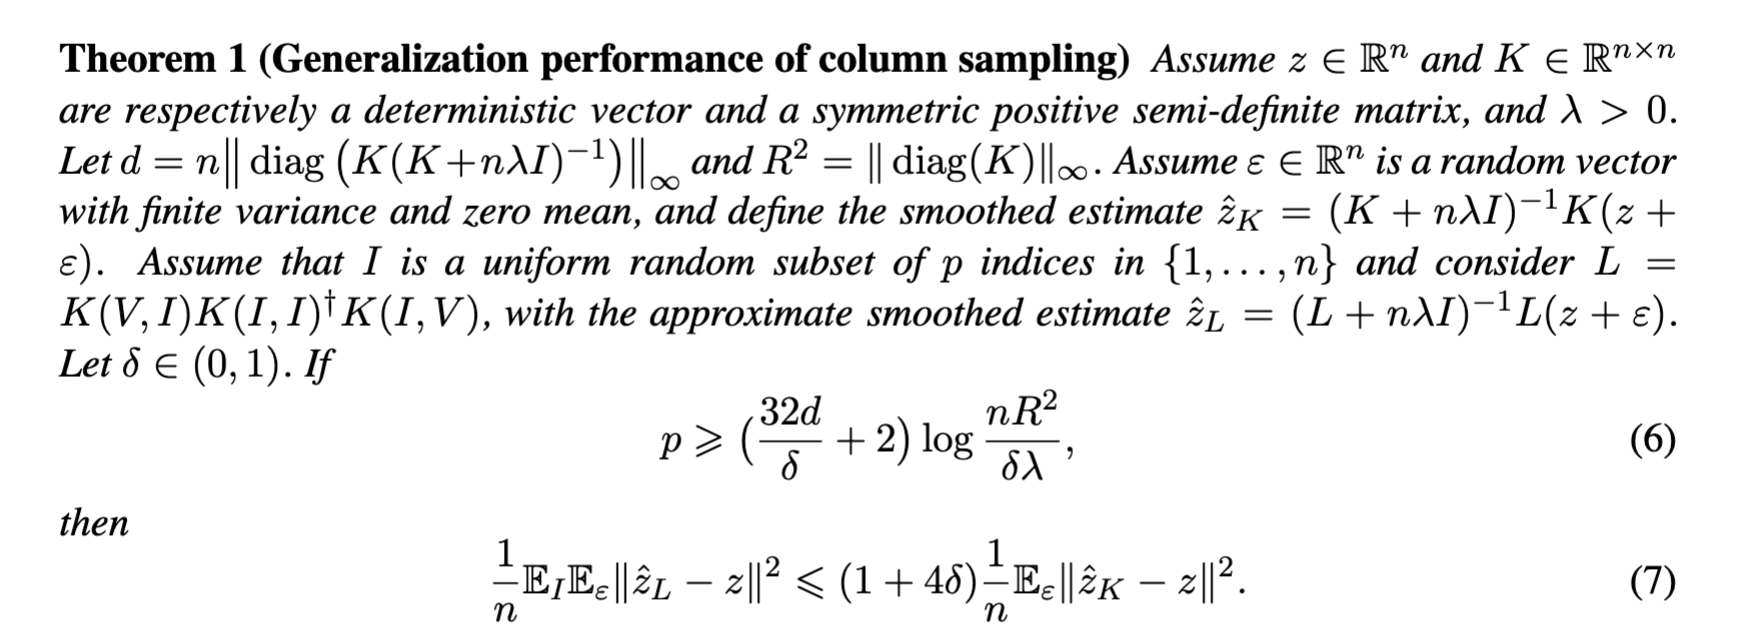
\includegraphics[width=1.05\textwidth]{11-kernel-survey/theorem_1.png}
        \centering
    \end{figure}
\end{frame}


\begin{frame}
    \frametitle{Some observations}

    \begin{itemize}
        \item Provides a relative approximation guarantee (small values of $\delta$). 
        \item $p$ seen to by large in practise $\dots$
        \item Avoiding terms in $1/\lambda$. 
        \item Regularization effects.  
    \end{itemize}
\end{frame}

\begin{frame}
    \frametitle{Optimal choice of the regularization parameter}

    \begin{itemize}
        \item Based on eigenvalues and $n$.
        \item Provide some simulations. 
    \end{itemize}
\end{frame}